
\documentclass[convert={density=400,size=750x600,outext=.png},dvipsnames]{standalone}
\usepackage{tikz,amstext,bm,amssymb,paralist}
%%%pdflatex -shell-escape filename.tex
\usetikzlibrary{
  backgrounds,fit,positioning,shapes,shapes.arrows,
  decorations.pathreplacing,
  arrows,calc,decorations.markings,matrix}
\tikzstyle{block}=[align=flush center, draw=black, thick, rectangle, rounded corners=3pt]
\tikzstyle{codenode}=
  [block, rectangle split, rectangle split parts=2]
\tikzstyle{control point}=
  [codenode, very thick, rectangle split part fill={green!10,none}, draw=green!50!black]
\tikzset{
  big arrow/.style={
    decoration={markings,mark=at position 0.9999 with {\arrow[scale=1]{latex}}},
    postaction={decorate},
    shorten >=0.4pt}}

\tikzstyle{external code}=[top color=red!10, bottom color=red!30]
\tikzstyle{external area}=[top color=brown!10, bottom color=brown!30]
\tikzstyle{my code}=[top color=blue!10, bottom color=blue!30]
\tikzstyle{element}=[block, diamond, rounded corners=0pt, top
color=white, bottom color=gray!60]

\tikzstyle{wide box}=[block,minimum height=1cm,minimum width=3.5cm]
\tikzstyle{box}=[block,minimum height=1cm,minimum width=2cm]
\tikzstyle{my arrow}=[->, >=latex, thick, rounded corners=5pt]
\tikzstyle{transform arrow}=[my arrow, very thick]
\begin{document}
\sffamily
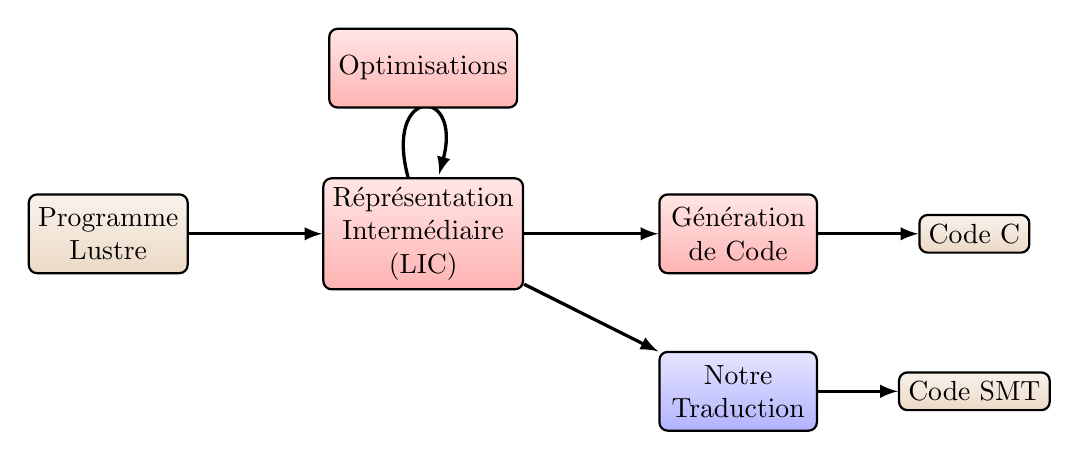
\begin{tikzpicture}[align=center]
\draw                     node[box,external area] (SeqProg) {Programme\\Lustre} ;

\draw (SeqProg) ++(4,0) node[box,external code](IntRepr)
{R\'{e}pr\'{e}sentation \\Interm\'{e}diaire \\ (LIC)};


\draw (IntRepr) ++(4,0) node[box,external code] (CodeGen)
{G\'{e}n\'{e}ration \\ de Code};

\draw (CodeGen) ++(0,-2) node[box,my code] (CodeGenSMT)
{Notre \\ Traduction};


\draw[transform arrow] (IntRepr) -- (CodeGen);
\draw[transform arrow] (IntRepr) -- (CodeGenSMT);
\draw[transform arrow] (SeqProg) -- (IntRepr);

\draw[transform arrow] (IntRepr) edge[loop above] node[box,external code](optim) {Optimisations} (IntRepr);
\draw (IntRepr) ++(0,1) ;


\draw (CodeGen) ++(3,0) node[block, external area] (cfile) {Code C} ;
\draw (CodeGen) ++(3,-2) node[block,external area] (smtfile) {Code SMT} ;

\draw[transform arrow] (CodeGen) to (cfile);
\draw[transform arrow] (CodeGenSMT) to (smtfile);



\end{tikzpicture}

\end{document}
